`% !TeX root = ../defense.tex

\section{Motivation}
\frame{\sectionpage}

\begin{frame}{Relative Turn Length}{Timing Diagram}
\begin{center}
\begin{tikzpicture}
 %   \begin{axis}[
 %       tumaxisstyle,
 %       x post scale=1.75,
     %   ymin=0,ymax=3,
 %        xmin=0,xmax=24,
 %        xlabel={Time}]
     %   ylabel={Turns}]
 %    \end{axis}
    \draw [->, thick, black] (0,0) -- (12.5,0);
    \draw (0,-.2) -- (0, .2);
    \draw (0.5,-.2) -- (0.5, .2);
    \draw (1,-.2) -- (1, .2);
    \draw (1.5,-.2) -- (1.5, .2);
    \draw (2,-.2) -- (2, .2);
    \draw (2.5,-.2) -- (2.5, .2);
    \draw (3,-.2) -- (3, .2);
    \draw (3.5,-.2) -- (3.5, .2);
    \draw (4,-.2) -- (4, .2);
    \draw (4.5,-.2) -- (4.5, .2);
    \draw (5,-.2) -- (5, .2);
    \draw (5.5,-.2) -- (5.5, .2);
    \draw (6,-.2) -- (6, .2);
    \draw (6.5,-.2) -- (6.5, .2);
    \draw (7,-.2) -- (7, .2);
    \draw (7.5,-.2) -- (7.5, .2);
    \draw (8,-.2) -- (8, .2);
    \draw (8.5,-.2) -- (8.5, .2);
    \draw (9,-.2) -- (9, .2);
    \draw (9.5,-.2) -- (9.5, .2);
    \draw (10,-.2) -- (10, .2);
    \draw (10.5,-.2) -- (10.5, .2);
    \draw (11,-.2) -- (11, .2);
    \draw (11.5,-.2) -- (11.5, .2);
    \draw (12,-.2) -- (12, .2);

    \draw (17,-.2) -- (17, .2);

    \node at (-1,-0.5) {Time};
    \node at (0,-0.5) {0};
    \node at (1,-0.5) {1};
    \node at (2,-0.5) {2};
    \node at (3,-0.5) {3};
    \node at (4,-0.5) {4};
    \node at (5,-0.5) {5};
    \node at (6,-0.5) {6};
    \node at (7,-0.5) {7};
    \node at (8,-0.5) {8};
    \node at (9,-0.5) {9};
    \node at (10,-0.5) {10};
    \node at (11,-0.5) {11};
    \node at (12,-0.5) {12};

    \node at (-1,1) {A};
    \node at (-1,2.5) {B};

    %A turn 1 , 0 - 1.5 sec with one da
    \uncover<1->{%
      \path [fill=gray] (0,0.5) rectangle (1.5,1.5);
    }

    \uncover<2->{%
        \draw [<->] (0,2.2) -- node[above] {T1} (1.5,2.2);
        \draw [<->] (0,1.6) -- node[above] {da1} (1.5,1.6);
    }

    %B turn 1, da1  2 - 3
    \uncover<3->{%
       \path [fill=teal] (2,2) rectangle (3,3);
       \draw [<->] (2,3.2) -- node[above] {da1} (3,3.2);
    }


    %B turn 1, da2 3.2 - 4
    \uncover<4->{%
        \path [fill=teal] (3.2,2) rectangle (4,3);
        \draw [<->] (3.2,3.2) -- node[above] {da2} (4,3.2);
    }

    \uncover<5->{%
            \draw [<->] (2,4) -- node[above] {T1} (4,4);
    }


    % A turn 2 4.5 - 6
    \uncover<6->{%
       \path [fill=gray] (4.5,0.5) rectangle (6,1.5);
    }

    % A turn 2 4.5 - 6 , header
    \uncover<7->{%
        \draw [<->] (4.5,2.2) -- node[above] {T2} (6,2.2);
        \draw [<->] (4.5,1.6) -- node[above] {da2} (6,1.6);
    }


    %B turn 2 6.5 - 7.5
    \uncover<8->{%
       \path [fill=teal] (6.5,2) rectangle (7.5,3);
    }

    %B turn 2 6.5 - 7.5 header
    \uncover<9->{%
        \draw [<->] (6.5,3.2) -- node[above] {da3} (7.5,3.2);
        \draw [<->] (6.5,4) -- node[above] {T2=1 sec} (7.5,4);
    }

    %A turn 3, da3=0.5, avg turn length: 1.5, RTL = 0.5/1.5
    \uncover<10->{%
       \path [fill=gray] (8,0.5) rectangle (8.5,1.5);
       \draw [<->] (8,1.6) -- node[above] {da3} (8.5,1.6);

    }

    \only<10> {
       \node at (11,3) {\small{Avg Turn Legnth: 1.5}};
       \node at (11,3.5) {\small{Relative Turn Legnth: $33\%$}};
       \draw [<->] (8,2.2) -- node[above] {\small{0.5 sec}} (8.5,2.2);
    }

    %A turn 3, da4, avg turn length: 1.5, RTL = 2/1.5
    \uncover<11->{%
       \path [fill=gray] (8.7,0.5) rectangle (10.3,1.5);
       \draw [<->] (8.7,1.6) -- node[above] {da4} (10.3,1.6);
    }

    \only<11> {
       \node at (11,3) {\small{Avg Turn Legnth: 1.5}};
       \node at (11,3.5) {Relative Turn Legnth: $153\%$};
       \draw [<->] (8,2.2) -- node[above] {\small{2.3 sec}} (10.3,2.2);

    }


    \uncover<12->{% avg turn length: 1.5, RTL = 3/1.5
       \path [fill=gray] (10.5,0.5) rectangle (11.5,1.5);
       \draw [<->] (10.5,1.6) -- node[above] {da5} (11.5,1.6);
    }

    \only<12> {
       \node at (11,3) {\small{Avg Turn Legnth: 1.5}};
       \node at (11,3.5) {Relative Turn Legnth: $233\%$};
       \draw [<->] (8,2.2) -- node[above] {\small{3.5 sec}} (11.5,2.2);

    }

\end{tikzpicture}
\end{center}
\end{frame}



\begin{frame}{Relative Floor Control}{Timing Diagram}
\begin{center}
\begin{tikzpicture}
 %   \begin{axis}[
 %       tumaxisstyle,
 %       x post scale=1.75,
     %   ymin=0,ymax=3,
 %        xmin=0,xmax=24,
 %        xlabel={Time}]
     %   ylabel={Turns}]
 %    \end{axis}
    \draw [->, thick, black] (0,0) -- (12.5,0);
    \draw (0,-.2) -- (0, .2);
    \draw (0.5,-.2) -- (0.5, .2);
    \draw (1,-.2) -- (1, .2);
    \draw (1.5,-.2) -- (1.5, .2);
    \draw (2,-.2) -- (2, .2);
    \draw (2.5,-.2) -- (2.5, .2);
    \draw (3,-.2) -- (3, .2);
    \draw (3.5,-.2) -- (3.5, .2);
    \draw (4,-.2) -- (4, .2);
    \draw (4.5,-.2) -- (4.5, .2);
    \draw (5,-.2) -- (5, .2);
    \draw (5.5,-.2) -- (5.5, .2);
    \draw (6,-.2) -- (6, .2);
    \draw (6.5,-.2) -- (6.5, .2);
    \draw (7,-.2) -- (7, .2);
    \draw (7.5,-.2) -- (7.5, .2);
    \draw (8,-.2) -- (8, .2);
    \draw (8.5,-.2) -- (8.5, .2);
    \draw (9,-.2) -- (9, .2);
    \draw (9.5,-.2) -- (9.5, .2);
    \draw (10,-.2) -- (10, .2);
    \draw (10.5,-.2) -- (10.5, .2);
    \draw (11,-.2) -- (11, .2);
    \draw (11.5,-.2) -- (11.5, .2);
    \draw (12,-.2) -- (12, .2);

    \draw (17,-.2) -- (17, .2);

    \node at (-1,-0.5) {Time};
    \node at (0,-0.5) {0};
    \node at (1,-0.5) {1};
    \node at (2,-0.5) {2};
    \node at (3,-0.5) {3};
    \node at (4,-0.5) {4};
    \node at (5,-0.5) {5};
    \node at (6,-0.5) {6};
    \node at (7,-0.5) {7};
    \node at (8,-0.5) {8};
    \node at (9,-0.5) {9};
    \node at (10,-0.5) {10};
    \node at (11,-0.5) {11};
    \node at (12,-0.5) {12};

    \node at (-1,1) {A};
    \node at (-1,2.5) {B};

    %A turn 1 , 0 - 1.5 sec with one da
    \uncover<1->{%
      \path [fill=gray] (0,0.5) rectangle (1.5,1.5);
      \draw [<->] (0,2.2) -- node[above] {T1} (1.5,2.2);
      \draw [<->] (0,1.6) -- node[above] {da1} (1.5,1.6);
      \path [fill=teal] (2,2) rectangle (3,3);
      \draw [<->] (2,3.2) -- node[above] {da1} (3,3.2);
      \path [fill=teal] (3.2,2) rectangle (4,3);
      \draw [<->] (3.2,3.2) -- node[above] {da2} (4,3.2);
      \draw [<->] (2,4) -- node[above] {T1} (4,4);
    }

    %Total Length
    \only<1> {
        \draw [<->] (0,4.7) -- node[above] {\small{4 sec}} (4,4.7);
    }


    % A turn 2 4.5 - 6
    \uncover<2->{%
       \path [fill=gray] (4.5,0.5) rectangle (6,1.5);
       \draw [<->] (4.5,2.2) -- node[above] {T2} (6,2.2);
       \draw [<->] (4.5,1.6) -- node[above] {da2} (6,1.6);
    }

    %Total Length
    \only<2> {
        \node at (11,4) {\small{A RTC: 1.5}};
        \node at (11,3) {\small{B RTC: 1.5}};
        \draw [<->] (0,4.7) -- node[above] {\small{6 sec}} (6,4.7);
    }

    %B turn 2 6.5 - 7.5
    \uncover<3->{%
       \path [fill=teal] (6.5,2) rectangle (7.5,3);
       \draw [<->] (6.5,4) -- node[above] {T2} (7.5,4);
    }

        %Total Length
    \only<3> {
        \node at (11,4) {\small{A RTC: 2}};
        \node at (11,3) {\small{B RTC: 2}};
        \draw [<->] (0,4.7) -- node[above] {\small{7.5 sec}} (7.5,4.7);
    }


    %A turn 3, da3=0.5, avg turn length: 1.5, RTL = 0.5/1.5
    \uncover<4->{%
       \path [fill=gray] (8,0.5) rectangle (8.5,1.5);
       \draw [<->] (8,1.6) -- node[above] {da3} (8.5,1.6);

    }

    \only<4> {
        \node at (11,4) {\small{A RTC: 2}};
        \node at (11,3) {\small{B RTC: 2}};
        \draw [<->] (0,4.5) -- node[above] {\small{8 sec}} (8,4.5);
    }

    %A turn 3, da4, avg turn length: 1.5, RTL = 2/1.5
    \uncover<5->{%
       \path [fill=gray] (8.7,0.5) rectangle (10.3,1.5);
       \draw [<->] (8.7,1.6) -- node[above] {da4} (10.3,1.6);
    }

    \only<5> {
        \node at (11,4) {\small{A RTC: 3}};
        \node at (11,3) {\small{B RTC: 3}};
        \draw [<->] (0,4.5) -- node[above] {\small{10.3 sec}} (10.3,4.5);
    }


    \uncover<12->{% avg turn length: 1.5, RTL = 3/1.5
       \path [fill=gray] (10.5,0.5) rectangle (11.5,1.5);
       \draw [<->] (10.5,1.6) -- node[above] {da5} (11.5,1.6);
    }

    \only<12> {
       \node at (11,4) {\small{A RTC: 4}};
       \node at (11,3) {\small{B RTC: 4}};
        \draw [<->] (0,4.5) -- node[above] {\small{11.4 sec}} (11.5,4.5);
    }

\end{tikzpicture}
\end{center}
\end{frame}




\begin{frame}{Current Issues}
    \begin{enumerate}[<+->]\itemsep9pt
      \item For a natural conversation between human and machine, we want to conform
            to human to human turn taking system (Sacks et al, 1978)
      \item In Human-Human conversations conversant predict (Sacks et al, 1978) or
            signal (Duncan 1972) each other on coming turn transition
      \item {
        Timeouts leads to poor user interaction(Arsikere et al, 2015)
        \begin{itemize}
            \item Not effective in noisy environment
            \item too little - machine barge in during intra turn pause.
            \item too much - user waiting for the machine.
        \end{itemize}
      }
      \item {
        Turn transition prediction based on local features improve turn taking but still
        do not match human performance.
        \begin{itemize}
            \item Syntactic (Sacks et al 1978,De Ruiter et al. 2006)
            \item Prosodic (Ford 1996,Stolcke 2002,Ferrer 2003)
            \item Pragmatic (Ford 2001)
        \end{itemize}
      }
    \end{enumerate}
\end{frame}

\begin{frame} {Thesis Statement}
 \begin{center}

        \Large{Conversant's past behavior can help predict turn transitions}\\
        \vspace{10mm}
        \Large{Past behavior represented by Summary features}
 \end{center}

\end{frame}
